\documentclass{ctexart}

\usepackage{bookmark}
\usepackage{listings}
\renewcommand\figurename{Figure} 
\renewcommand\tablename{Table} 
\renewcommand\refname{References}
\CTEXsetup[format={\Large\bfseries}]{section}

\setmainfont{Times New Roman}

% 控制段首不缩进
\usepackage{parskip}
\setlength{\parindent}{0cm}

\renewcommand{\thefootnote}{\fnsymbol{footnote}}

\usepackage{amsthm}
\usepackage{abstract}
\usepackage{amsmath}

\usepackage{amssymb}

\usepackage{graphicx}

\usepackage{hyperref}

\usepackage[table]{xcolor}

\usepackage{fancyhdr}

\usepackage{lastpage}

\usepackage{pythonhighlight}

\usepackage{subfigure}

\usepackage{fancyhdr}

\usepackage{cite}

\usepackage{geometry}
\setlength{\absleftindent}{0pt}
\setlength{\absrightindent}{0pt} 
\geometry{left=3cm,right=3cm,top=1cm,bottom=1.5cm}
\begin{document}
\title{\textbf{MA263  概率论与数理统计大作业}}
\author{薛昊天 518021910506}
\date{}
\maketitle
\section{\textbf{问题1}}
\subsection{题目描述}
    $X{\sim}N(\mu_1, \sigma_1^{2})$, $Y{\sim}N(\mu_2, \sigma_2^{2})$, $\eta\sim{B(1, p)}$
    则有$Z = X + \eta{Y}$服从混合高斯分布。利用以上规则生成10000个数据,画出频率分布直方图。改变参数,观察频率分布直方图的“峰”的变化。

\section{实验及结论}
    利用Numpy库的random函数可以生成服从任意参数的正态分布随机数,以及服从0-1分布的随机数。根据题目描述生成10000个Z的数值,
再利用Matplotlib.pylab库中的hist功能可以画出频率分布直方图。
  \subsection{0-1分布中p对图像的影响}

   \centerline{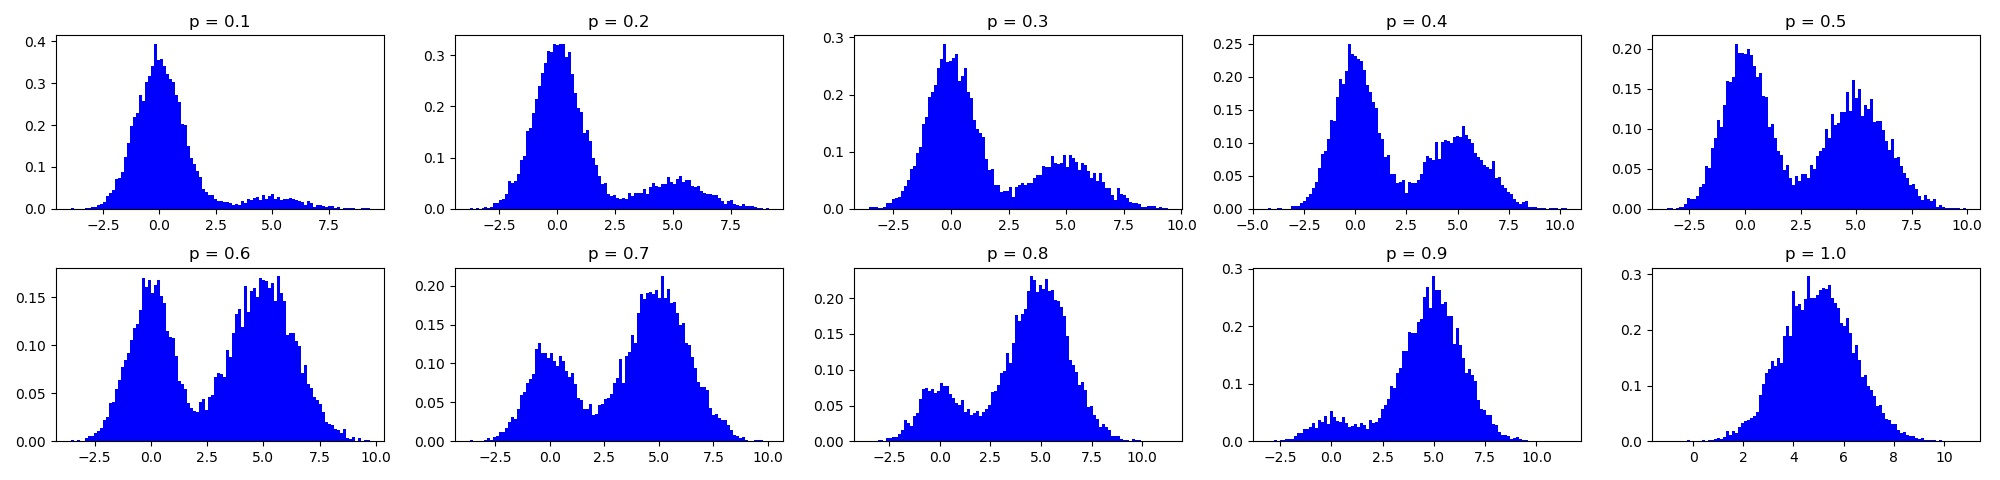
\includegraphics[scale=0.3]{pic_data/fig_gaitong2.jpg}}
   \centerline{图1}

   由于p对于和式中的$\eta{Y}$有着直接的影响,这里不是一般性,固定其它所有变量。
   可以从图1中看出,p很小的时候,图像几乎只体现为X的分布特点;随着p值逐渐增大,
   图像的峰变为两个且左边的峰逐渐减弱而右边的峰逐渐增大,随后当p=1时,两个峰趋于中和且峰值对应的横坐标点位于$\mu1+\mu2$处。
   \subsection{$\mu$对图像的影响}
   $\mu$是正态分布中的均值,图像上反应的正态分布峰值横坐标的值,在这里不失一般性,固定其它变量,只改变$\mu{2}$。

  \centerline{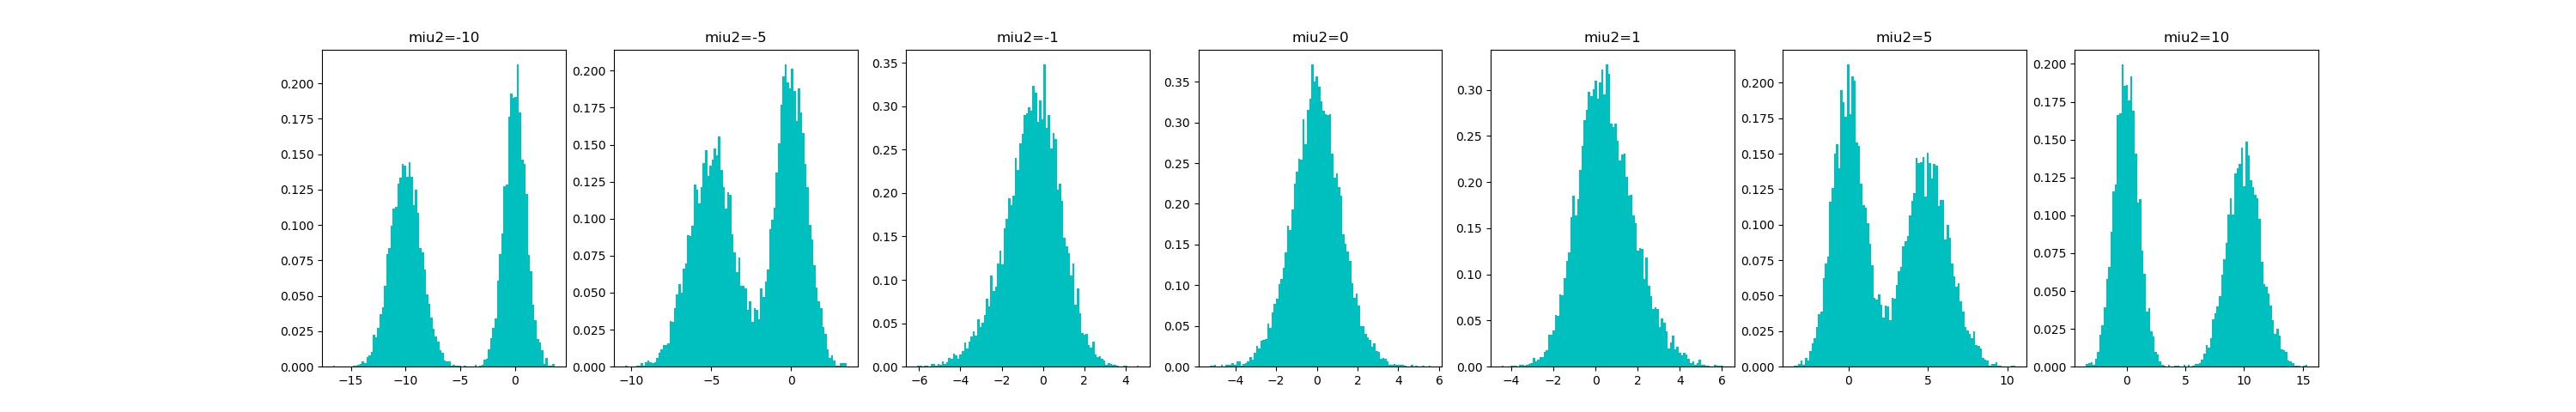
\includegraphics[scale=0.28]{pic_data/fig_miu.jpg}}
  \centerline{图2}
改变时Y变量的均值从-5到10,我们可以从图2中看出,Y所对应的峰值的坐标从-5到10移动,中途“穿过”了X所对应的
峰,且可以看出途中两个峰的高度基本保持不变,X对应的峰位置基本保持不变。
   \subsection{$\sigma$对图像的影响}
    和2.2的研究方法一致
    \subsubsection{只改变$\sigma1$}
    \centerline{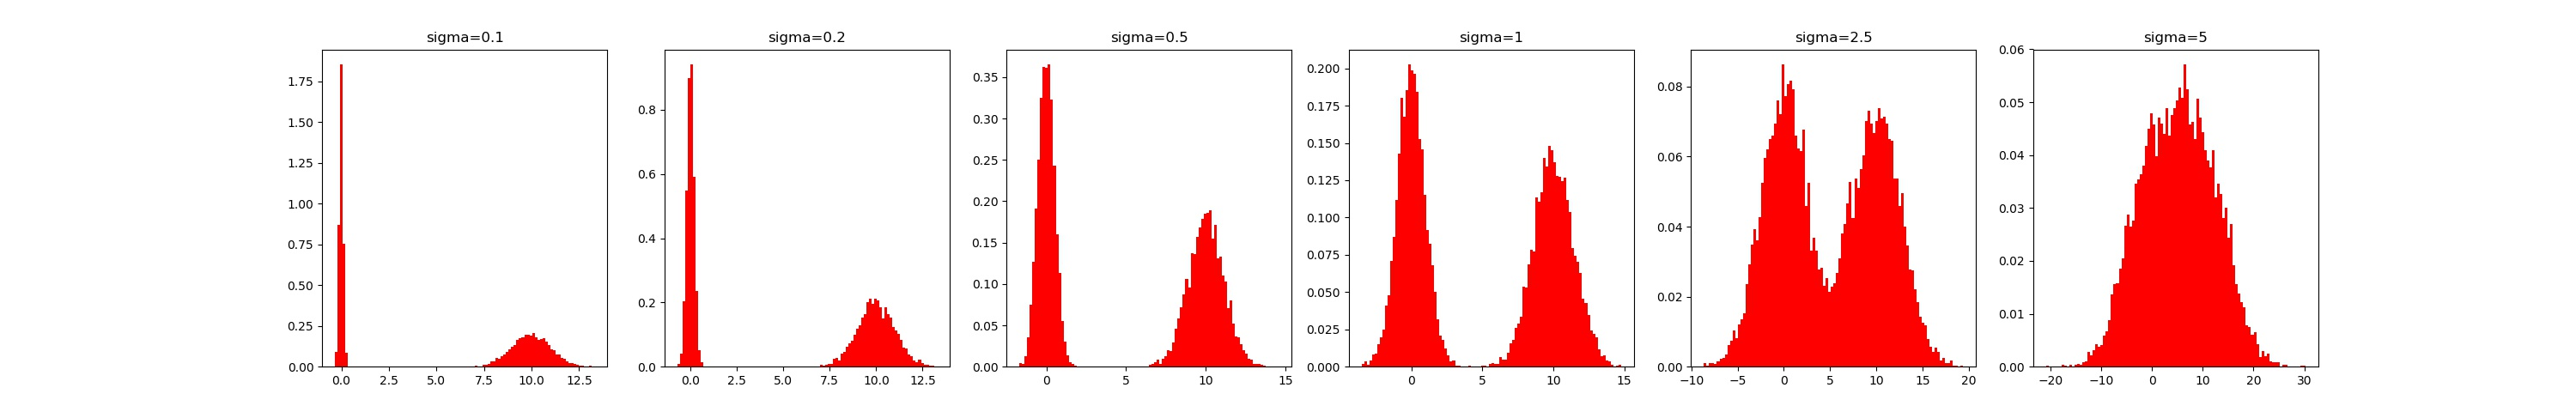
\includegraphics[scale=0.3]{pic_data/fig_sigma(fixed2).jpg}}
    \centerline{图3.1}
    从图3.1中可以看出:当X的方差很小的时候,左边峰也就是X变量所对应的峰就会很“尖”,此时右边Y
    所对应的峰很平。当X的方差逐渐变大后,左边的峰逐渐趋平,而右边的峰逐渐变尖,峰值逐渐变大;最后两个峰合成一个
    峰。
    \subsubsection{只改变$\sigma2$}
    \centerline{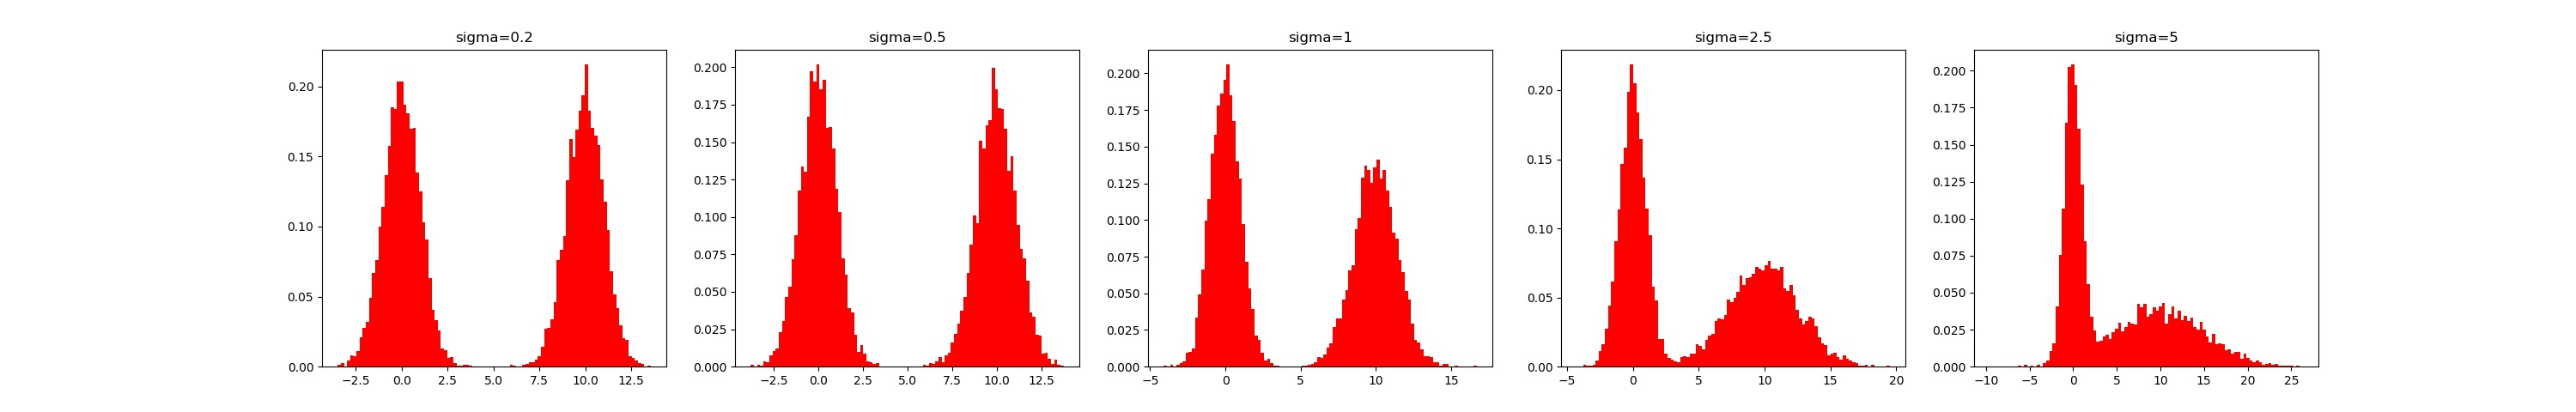
\includegraphics[scale=0.3]{pic_data/fig_sigma(fixed1).jpg}}
    \centerline{图3.2}
    如图3.2,和3.1类似。当Y的方差逐渐变大的时候,右边的峰变矮变平,左边的峰值保持不变,变尖。最后当方差足够大,一定会
    合二为一(图中为完全体现,但事实如此)。

    \section{问题2}
    \subsection{题目描述}
      自己设定参数,用计算机生成1000组,每组n个混合高斯分布随机数:第i组为$(Z_{i, 1}, Z_{i, 2}, ..., Z_{i, n})$
      \begin{equation*}
        U_i = \frac{\sum_{k=1}^{n}Z_{i, k} - nEZ}{\sqrt{nDZ}}
      \end{equation*}
      画出$U_1, U_2, ... U_1000$的频率分布直方图,讨论不同n对峰的影响。
    \subsection{实验以及结论}
    按照题目要求, 设定$\mu{1}=0,\mu2=5,\sigma{1}=\sigma{2}=1,p=0.5$分别取n = 20, 50, 100, 1000画出频率分布直方图。可以看出
    当n很小的时候图像十分离散,有很多不连续峰。当n越大的时候,U的分布
    越来越趋向于正态分布。且由中心极限定律可以知道当n足够大的时候,U趋向于标准正态分布。所以我们可以得出,当n很大时,随机量相互抵消,
    最后近似服从标准正态分布,这也正是中心极限定律的思想。
    \begin{figure}[htbp]
  \centering
    \subfigure[n = 20]{
      \begin{minipage}[t]{0.3\linewidth}
        \centering
        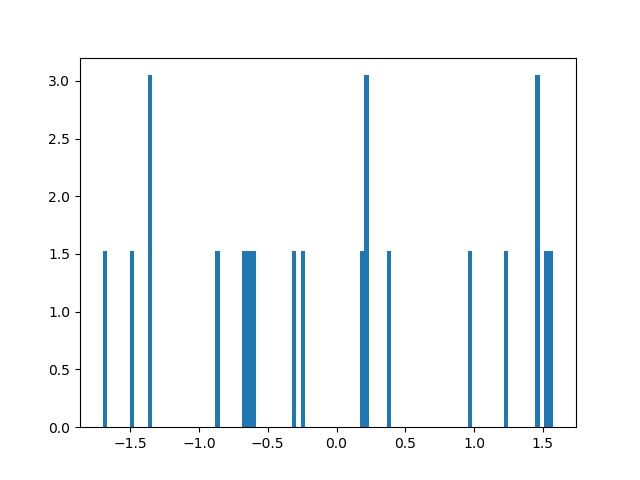
\includegraphics[scale = 0.3]{pic_data/Q2(20).jpg}
      \end{minipage}
    }
    \subfigure[n = 50]{
      \begin{minipage}[t]{0.3\linewidth}
        \centering
        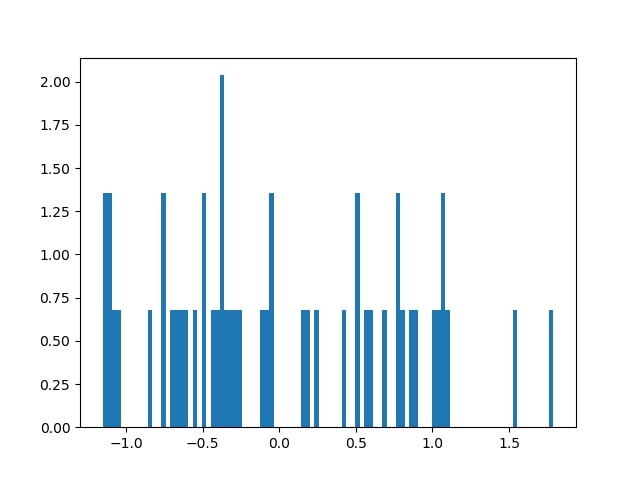
\includegraphics[scale = 0.3]{pic_data/Q2(50).jpg}
      \end{minipage}
    }


    \subfigure[n = 100]{
      \begin{minipage}[t]{0.3\linewidth}
        \centering
        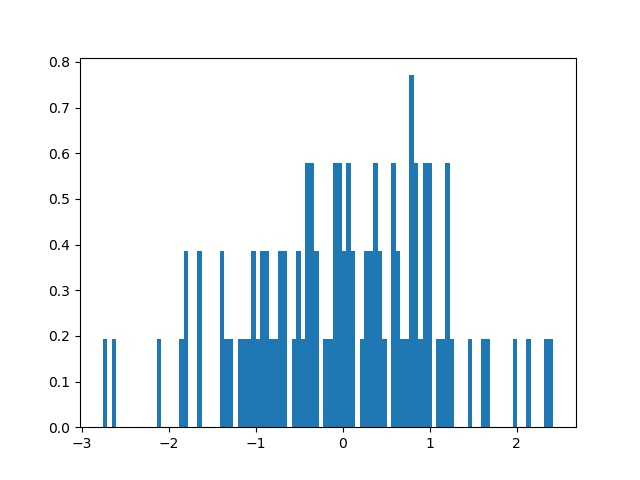
\includegraphics[scale = 0.3]{pic_data/Q2(100).jpg}
      \end{minipage}
    }
    \subfigure[n = 1000]{
      \begin{minipage}[t]{0.3\linewidth}
        \centering
        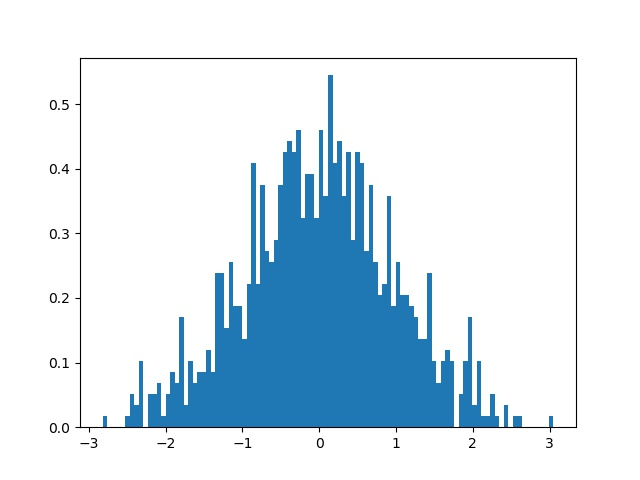
\includegraphics[scale = 0.3]{pic_data/Q2(1000).jpg}

      \end{minipage}
    }
\end{figure}
\section{致谢}
  感谢熊老师上课详细的理论知识的介绍,感谢老师助教以及同学们课后的答疑解惑。 

  
    \end{document}